\documentclass[conference]{IEEEtran}
\usepackage{graphicx}
\usepackage{amsmath}
\usepackage{amssymb}
\usepackage{subfig}
\usepackage{wrapfig}

\usepackage[font=small,labelfont=bf]{caption}

\usepackage{array}

\usepackage{comment}

\newcolumntype{P}[1]{>{\centering\arraybackslash}p{#1}}
\newcolumntype{M}[1]{>{\centering\arraybackslash}m{#1}}

\newcommand{\ie}{{\em i.e.}}
\newcommand{\eg}{{\em e.g.}}
\newcommand{\et}{{\em et al.~}}
\newcommand{\real}{\mathbb{R}}
\newcommand{\integer}{\mathbb{N}}

\newtheorem{theorem}{Theorem}
\newtheorem{lemma}{Lemma}
\newtheorem{corollary}{Corollary}
\newtheorem{definition}{Definition}

\renewcommand{\refname}{\centerline{References cited}}
\newcommand{\required}[1]{\section*{\hfil #1\hfil}}

% this handles hanging indents for publications
\def\rrr#1\\{\par
\medskip\hbox{\vbox{\parindent=2em\hsize=6.12in
\hangindent=4em\hangafter=1#1}}}

\def\baselinestretch{1}

\begin{document}

\title{\LARGE\bf %Narrow Down the Root Cause of Integrity Errors for Networked Systems
Root Cause Localization of Data Integrity Errors in Internet Scale Applications
\thanks{This work is supported by the
    US National Science Foundation through the NSF awards ACIXXX.}
}
\author{\IEEEauthorblockN{Yufeng Xin, Shih-Wen Fu, \\ Anirban Mandal, Ilya Baldin }
\IEEEauthorblockA{%RENCI\\
RENCI, UNC - Chapel Hill\\
Chapel Hill, NC, USA\\
}
\and
\IEEEauthorblockN{Mats Rynge, Karan Vahi, \\ Ewa Deelman}
\IEEEauthorblockA{%ISI\\
ISI, USC\\
Marina Del Rey, CA, USA\\
}
\and
\IEEEauthorblockN{Ishan Abhinit, Von Welch}
\IEEEauthorblockA{%CACR\\
CACR, Indiana University\\
Bloomington, IN, USA\\
}
}

\maketitle
\thispagestyle{empty}

\begin{abstract}
For large-scale distributed applications involving intensive data transfers over a network, root cause analysis (RCA) for error diagnosis becomes extremely challenging. One main reason is that the underneath network is often of multi-domain nature, where limited component level information is available, and where it is not possible to instrument and measure traffic flows at all the nodes in the network. It's hard, if not completely possible, to build proper system diagnosis models. As a result, RCA remains a guessing art that requires manual debugging and daunting amount of communication between operators from different domains and subsystems that often takes days or even weeks.  

Among the more challenging failure modes are the so-called ``grey failures" that only come to effect randomly, often at low probability. One such common failure mode is the integrity errors that may corrupt data, which is caused either by the storage subsystem or a network component along data transfer path. 

In this paper, we focus on the integrity error RCA problem in a networked system setting. We first cast it as a multi-label classification problem with the goal to enable root cause inference for a given network only from the flow level check at the end hosts. Collecting sufficient training data is fundamentally difficult with a machine learning approach, which is typical for production systems due to lack of monitoring services. We therefore built an emulation environment in a Cloud testbed that allows creating arbitrary large-scale virtual network systems. We further developed a suite of software tools to automate the training process that includes configuring the network routing, instrumenting data transfers between end hosts, injecting arbitrary integrity errors into the network components, and collecting and processing the raw data. This gives us extra benefits in experiment repeatability and efficiency. For evaluation, we trained several multi-label classification models and validated their performance with a Top-$k$ accuracy metric for an emulated network. The results demonstrate the efficacy of the approach and potential to apply the learned models to production systems.  

\end{abstract}

\section{Introduction}
\label{sec:introduction}
Root cause analysis (RCA) is a critical function in operating and managing complex networked systems, be it physical, software, or hybrid~\cite{RCA-Review-2017}.
It aims to identify the component(s) and process(es) responsible for the fault manifested by the wrong results or system failures in a timely fashion.
Traditional RCA relies on system domain models that can be used to deduce the potential component failures from the system symptoms and behaviors.
However, exponentially increasing system scale, complex component interdependencies, and lack of visibility in multi-domain, large-scale networks have 
significantly made it harder to build such models for efficient fault identification and localization for modern distributed systems. 
As a result, RCA in such a distributed and opaque system setting has drawn extensive research attention in recent years, which have found prominent uses
 in data center networks and Internet applications. Not surprisingly, these studies have adopted the machine learning (ML) or data analytic approaches
due to the relaxed requirements on accurate domain models~\cite{netbouncer:nsdi18,Link-JIoT-2019}.

In this paper, we take a new application domain, the scientific workflow management systems (WMS), as our primary motivating use case to tackle the complex
 system RCA problem using a machine learning approach. WMS facilitates in-order execution of jobs in workflows and includes large amounts of interdependent
  data transfers, storage functions, and computation tasks. These tasks are often distributed over distributed hardware, software, and data resources
   located in different facilities nationwide or globally. Inevitably, frequent system failures and reliability issues 
caused by errors and faults from underlying subsystems have been serious concerns for the WMS community. 
Therefore most WMS have built-in failure handling mechanisms like redundancy and automatic retries. 
They also try to provide as much log information as possible to help with failure diagnosis, which normally assumes a long manual process.

Since a typical workflow system runs as a middleware sitting several layers above the infrastructure resources that are managed 
and operated by different service providers (domains), it has a limited view of the health of the infrastructure components. 
Most critically, it has no direct knowledge of the exact path of the data movement,
sometimes even the sources and sinks are normally abstracted in virtual namespaces.  
Consequently, fault diagnosis, especially identifying the root cause of the failures becomes extremely difficult, and normally 
costs coordinated efforts and long hours from many operators of different sub-systems, often after many unsuccessful (and wasted) retries from the users. 
Hence, analyzing the root cause of failures for data integrity errors in distributed workflow executions is a representative yet very difficult problem.

In a nutshell, ML-based RCA can be formulated as a multi-class classification problem, where the potential root causes are the labels and various 
measurement and observations of the tasks and data flow level observations are used as the features.
RCA for large-scale networked systems poses other unique challenges in adopting ML approaches.
 
The first challenge comes from the prevalence of so-called {\it gray failures} in the networked system, in addition to the normal {\it stop failures}~\cite{GrayFailure:2017,DeepView:NSDI18}. A {\it stop failure} is a kind of hard failure, which refers to the complete breakdown of a component that disrupts all traffic flows or paths over this component deterministically~\cite{Link-JIoT-2019}. {\it Gray failures} are those probabilistic failures in a component that would act normally most of the time and that could not be caught by the traditional deterministic system monitoring and diagnostic tools. We categorize two types of  {\it gray failures}: performance degradation and data integrity errors. The former is normally caused by system overload that will lead to slow response, timeout, and the frequent reboot of the servers or software. The latter may randomly corrupt bits in a block of data or packets over network transfer. Since existing checksum mechanisms implemented in TCP and the storage services are not sufficient to guarantee end-to-end data integrity, they often get unnoticed for a long time until severe consequences to applications occurred. Therefore modern WMS have started to add end-to-end integrity check mechanisms, including in Pegasus~\cite{swip:pearc:2019} and Globus~\cite{IntegrityVerification:DataTransfer}.

The second challenge lies in the difficulties in acquiring sufficient training data feeds to a ML-based RCA system. For a system over the Internet, the global routing information is not completely available for the RCA system as they are normally proprietary to the different service providers (domains). The possible monitoring data sources or active probe sites in a network are always limited. As a result, in addition to passive monitoring data, active probes or event fault injections are often used to generate more diagnosis data~\cite{active:iot:2019, NetPoirot:Sigcomm2016}. Then, due to the desire of conducting RCA in real-time, how to minimize the overhead and latency of data collection in a production setting becomes a significant design issue.

The last but not the least challenge is to design and train the right ML models to achieve high diagnosis accuracy, out of a large pool of candidates~\cite{Boutaba:2018aa}. We will show that even the most basic questions of defining a data point, feature selection, and performance evaluation need special consideration.

In~\cite{Link-JIoT-2019}, the authors attempted to identify the stop failure of network links via the popular multi-class ML models using end-to-end passive traffic engineering measurements (throughput, latency, and packet loss). The authors in \cite{DeepView:NSDI18} took an active probe approach to localize the fault in a virtual disk system to the finest granularity up to the network switches. In~\cite{netbouncer:nsdi18}, a necessary condition was derived on the minimal set of paths that active probes need to be sent over the targeted network. The line of work including~\cite{NetPoirot:Sigcomm2016,KDD14} adapted a statistical learning approach to infer the probabilistic relationship between the path failure and the link faults. All these research works made a strong assumption that one can instrument probes or observations from any node to any other node in the network since their target systems are data center networks that they own. In an earlier study, the decision tree model was used to predict if a request will fail or succeed over a flawed network system~\cite{DT:2004}. Bayesian inference was demonstrated to be efficient for fast diagnosis when the causal relationship model is established in a large Internet system~\cite{BN-Internet:2007}.

In this paper, we first cast the WMS integrity error diagnosis as a networked system Root Cause Analysis (RCA) problem, where limited network system information is available for end-to-end data transfers (Section~\ref{sec:integrity}). Our main hypothesis is that the mapping between the endhost level flow statistics and the possible network component failures can be learned and inferred from a sufficiently large amount of labeled training data. In order to obtain sufficient training data and make repeatable experiments more efficient, we created an experimental system in a Cloud testbed that can automatically create a large-scale OSPF-enabled virtual network system, initiate data transfers between end hosts, and inject arbitrary integrity errors into the virtual router interfaces and end hosts (Section~\ref{sec:emulation}). We then studied several variants from three different families of multi-class classification models, Bayesian inference, SVM, and Decision Tree, and validated their accuracy performance using a Top-$k$ accuracy metric (Section~\ref{sec:ml}). With the data collected from the emulation, we evaluate their accuracy in Section~\ref{sec:evaluation}. We specifically studied the impact of available data transfer data in terms of end host pair coverage. We conclude the paper with our future research plan in Section~\ref{sec:future}.


\section{RCA for Network Integrity Errors}
\label{sec:integrity}
It has been recently recognized that existing protection mechanisms commonly implemented on Internet and distributed systems such as TCP checksums and redundant coding in storage systems are not sufficient to handle silent {\it gray failures}, which often leads to widespread system slowdown, application malfunction, and corrupted data. As a result, advanced distributed systems started to add extra end-to-end data integrity checks to catch these failures early on in order to reduce application failures and blind retries~\cite{swip:pearc:2019}. 

However, identifying the root causes of this type of gray failures remains a largely unsolved problem due to the challenges presented in Section~\ref{sec:introduction}: 
incomplete network state information, intermittent probabilistic nature of gray failures, and complexity in diagnosing complex networks in a scalable fashion.  

A network system can be modeled as a graph with a set of nodes connected by links via interfaces. The nodes in the network consist of end hosts (that generate and receive data) and networking devices (routers or switches that forward data). Due to scalability or privacy constraints, deploying monitoring capabilities at every point of the targeted large-scale network is not possible. Therefore, the problem can be concisely modeled as a bipartite mapping graph between the path level flows and its network components as shown in Fig.~\ref{fig:bipartite}. What makes the problem extremely more difficult is when the mapping relationships in the bipartite graph are unknown. We further observe that one component failure (e.g., $L_j$) will cause multiple paths erroneous while one flow error (e.g., $F_i$) may be caused by multiple component failures. And because the component gray failure probability is normally low ($10^{-3} - 10^{-6}$), it would require a large number of file transfers to catch a few corrupted files. Our ultimate goal is to localize the possible root causes in node or link errors by inference from the observed flow level abnormalities only at the end hosts, which can be translated to learning the mappings in such a graph.

\begin{wrapfigure}{ht}{0.25\textwidth}
  \begin{center}
    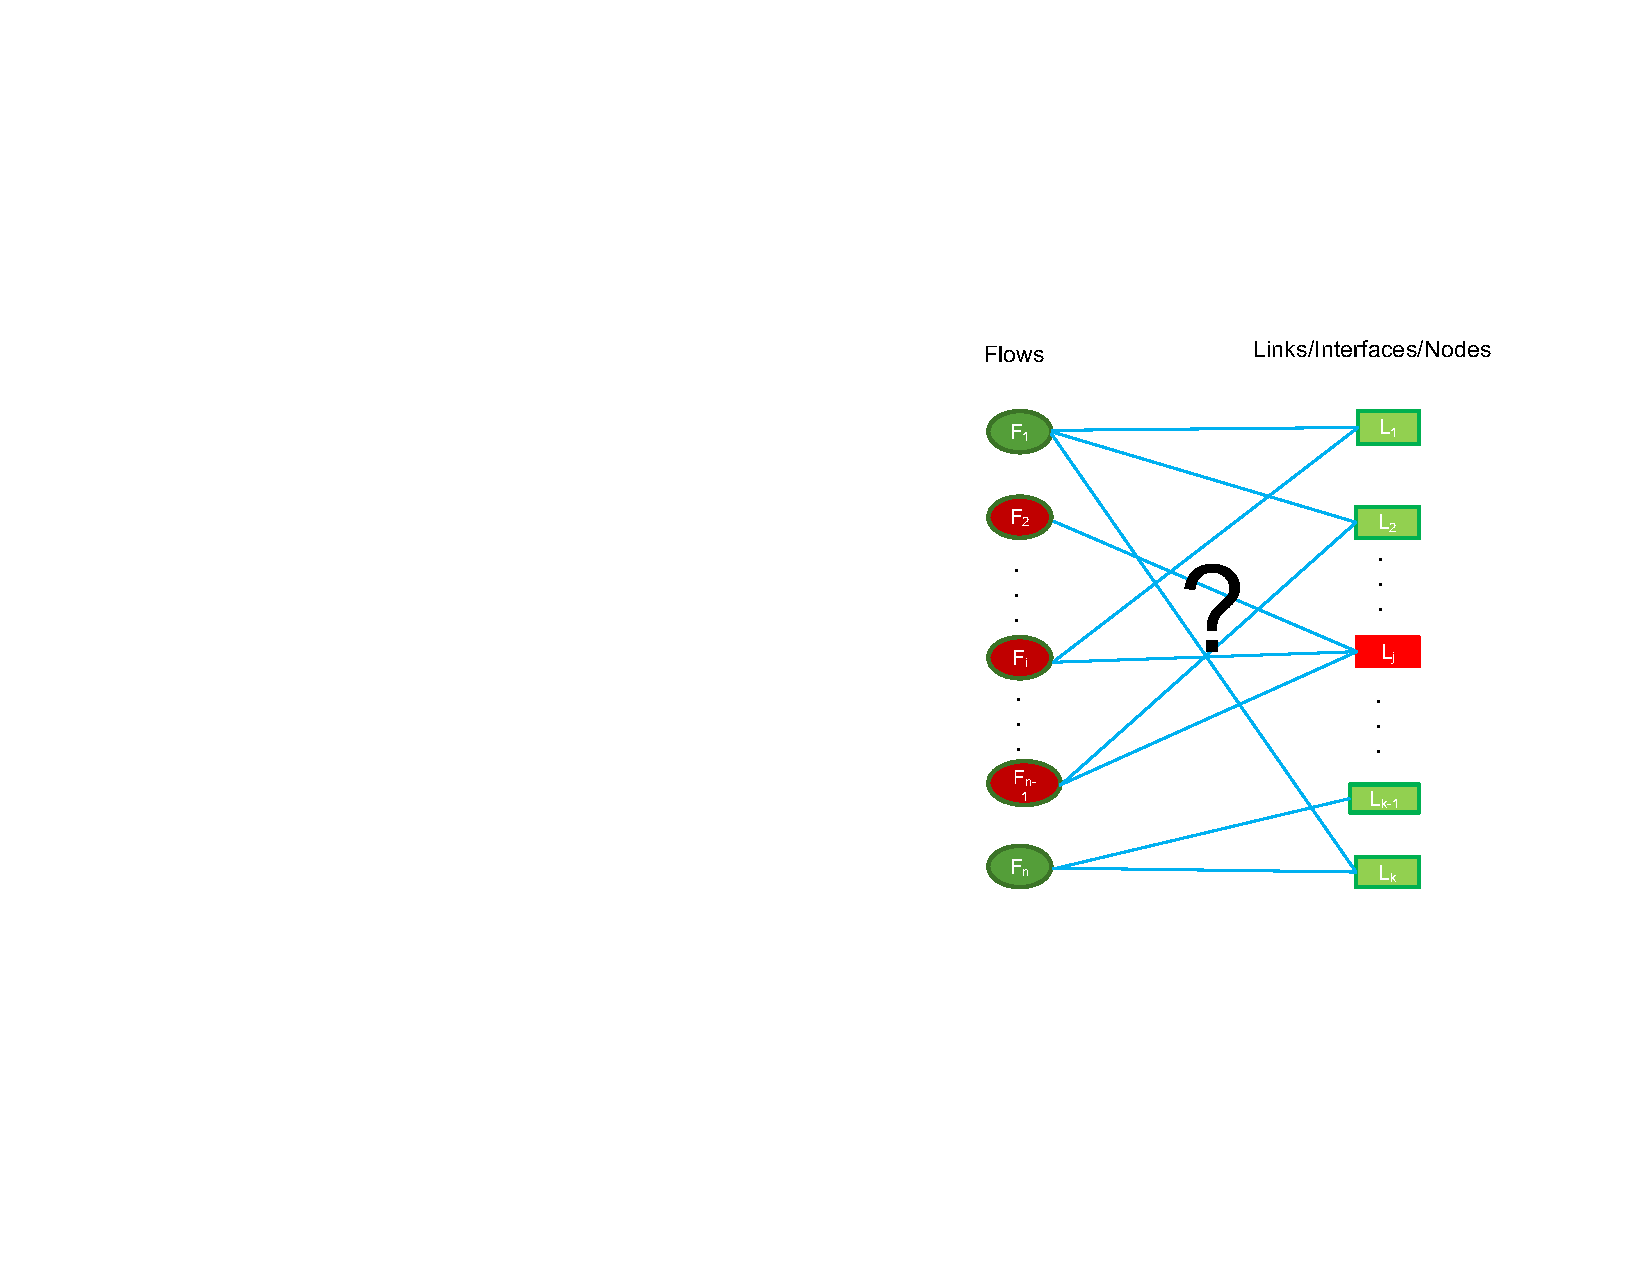
\includegraphics[width=0.25\textwidth]{./figure/RCABipartite}
  \end{center}
  \vspace{-5pt}
\caption{RCA Bipartite Graph}
\vspace{-5pt}
\label{fig:bipartite}
\end{wrapfigure}

The majority of recent studies assume flow information between any pair of nodes in the network is available because they focus on data center networks that they have full ownership and their modern routers allow originating and receiving probing data. This is very important because, as shown in~\cite{netbouncer:nsdi18}, there exists a minimal set of source-destination pairs to guarantee successful pinpointing of link errors in the network. They further assume the routes for all flows are known, i.e., the mapping represented in Fig.~\ref{fig:bipartite}. However, both assumptions do not hold for our targeted Internet environment due to obvious administrative constraints, complex topology, and the lack of monitoring coverage. In the Internet-scale network, traffic routing and forwarding paths are hard to obtain because of frequent topology and policy changes, the widely adaptation of multi-path routing, and disabled {\it Ping} and {\it Traceroute} in many places~\cite{arzani2018democratically}. Furthermore, deployment of a monitoring infrastructure to conduct system-wide active and passive monitoring is administratively and costly prohibitive.     

Therefore we made more restrictive but more realistic assumptions in this study in that (1) only the data file transfer information including integrity error states can be obtained at the end hosts from the application layer; (2) only the physical nodes (or abstract representation of domains) and their interfaces are known to us, but the network topology and traffic routing are unknown. 

In a large network, collecting the passive monitoring data from all node pairs may not scale well. Therefore, injecting probe packets between the designated node pairs periodically is adapted by several existing RCA systems. In practice, due to the probabilistic nature of the grey failures, controlled fault injection is an efficient way to generate training data within a reasonable time frame.

Directly accessing the production system to instrument the analysis with either active probing or fault injection is not realistic in most cases, especially in a multi-domain system where no one owns the entire infrastructure like in the data center networks. We believe emulation with realistic scales is a viable choice to train an efficient RCA model, given advanced Cloud testbeds are available.










\section{Network Emulation and Fault Injection}
\label{sec:emulation}
It's convenient to create an arbitrary virtual network system in an advanced Cloud testbed such as the NSF ExoGENI cloud testbed~\cite{ExoGENI:web}. Distributed applications, like Pegasus WMS, a popular WMS to coordinate the data transfer and compute job submission in such an environment with recently added end-to-end flow level integrity error checking capability can be installed and ran in the virtual network system~\cite{swip:pearc:2019}. The unit of data transfers is a {\it file} of different size for which we define as a {\it flow} from an origin end host to a destination end host. Pegasus can check the data integrity of flows at the end host.     

In order to simulate different types of sources of integrity errors, we added a new utility in Chaos Jungle~\cite{swip:pearc:2019,chaosjungle:web}, which can corrupt arbitrary file(s) in nodes in addition to packets out of network interfaces according to a given probability. This tool gives us the capability to inject controlled errors into any network elements using several integrity threat models~\cite{threat-model}.

The main design goal here is to automate the experiment creation, configuration, and data collection at any given scale in order to guarantee repeatable experiments at different scales and efficient data manipulation for ML model training. 
At the same time,  the emulated network could also be used as a sandbox to generate a high-fidelity RCA model for a production network system to use. 

\subsection{Network creation and configuration}
An arbitrary topology can be created on ExoGENI with nodes in the form of virtual machines (VM) running customized images. In our experimental topology, we use a set of end hosts to emulate the OSG data sources and sinks, a virtual network consisting of core routers emulating the backbone network service providers (Internet2, ESNet, etc.) and access routers emulating the access network service providers (regional research and education networks and campus networks). All nodes are connected with virtual layer-2 links with certain throughput guarantees in the private data plane. The end hosts run an Ubuntu image with our Chaos Jungle fault injection tools. The routers run an Ubuntu image with the Zebra software router and our Chaos Jungle fault injection tools. Using our automation software, an experimental system can be easily created with routing configured and network reachability established automatically through the APIs and the template scripting capability provided by ExoGENI.   

\subsection{Data transfer and fault injection}
For every experiment, we attach a controller node that can reach all the nodes in the topology via the management plane interface. The controller is provided a Postboot script that automatically learns the experimental topology, creates a list of end hosts, routers, and links, and populates the end hosts with a set of files for the data transfer.

A user can log into the controller node, modify the experimental configuration files that define the data origin and sink nodes, the list of nodes to introduce storage integrity error, the list of network link interfaces to be disrupted by the Chaos Jungle tool, and the fault injection probability.

Then the experiment software can be started to inject the fault, transfer the data files from the origins, check the integrity at the sinks, and collect the data. This sequence is repeated for every fault specified in the configuration file.

\subsection{Data collection and analysis}
At the last step, all the raw data will be processed and stored in the final result database files with predefined feature columns. Each database entry represents one data transfer with features of the file name, file size, origin, sink, access router, integrity error or not, etc. However, the forwarding path is unknown as it is controlled by the routing control plane process. The final result is exported to a Jupyter notebook environment where all the ML-based data analysis is performed.

The entire emulation process is fully automated via our software suite that includes bootstrapping the network, instrumenting data transfers, injecting integrity errors at chosen network elements, collecting and preprocessing the raw data. 

\begin{figure}[!ht]
\begin{center}
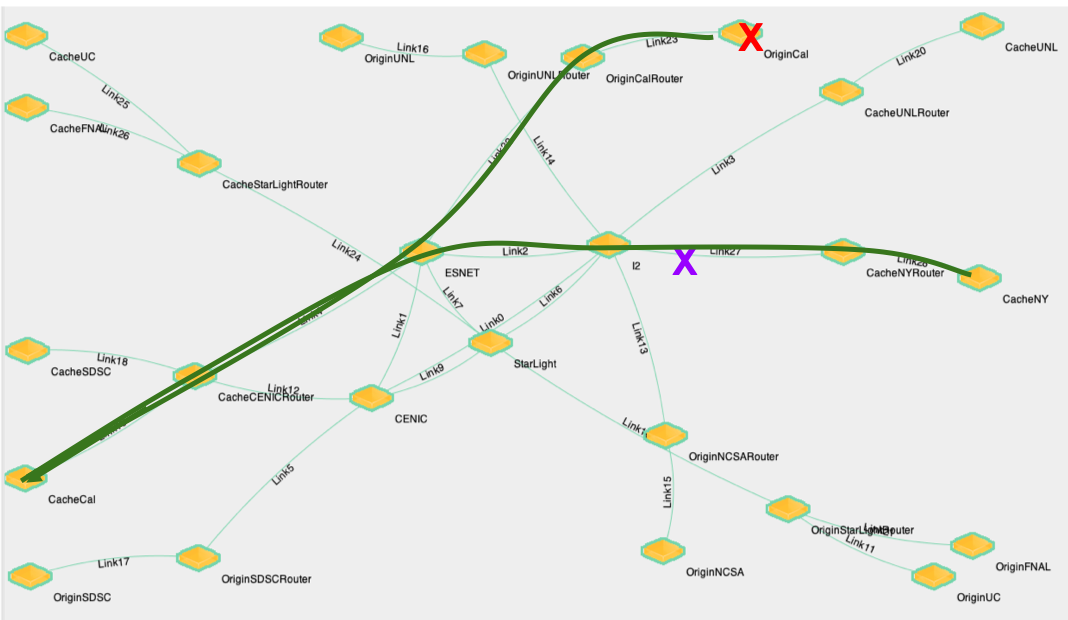
\includegraphics[width=0.48\textwidth]{./figure/ChaosJungle}
\end{center}
\caption{Experimental Topology}
\label{fig:topology}
\end{figure}

We use Fig. 2, an annotated screenshot from the ExoGENI GUI, to illustrate an emulated network system, a simplified version of the Open Science Grid (OSG) data federation network that is highly utilized to distribute data for high throughput scientific computing and is also a major infrastructure that Pegasus has been deployed~\cite{OSG:web}. This network consists of multiple end hosts running the data transfer and computing jobs controlled by Pegasus, and a set of routers in the middle to represent multiple forwarding domains. The two cross signs, one on an 
end host and another one on a network link, represent the locations where we inject the data integration errors with a probability setting. When an error is enabled (injected), all the traffic flows pass through the faulty element will be subject to possible data corruption as the error may flip the bits of packets randomly under a predefined probability. As we have discussed, most of these corrupted packets will not be caught by TCP or the storage system. As a results, some corrupted files will successfully land at the destination end hosts and will only be detected by Pegasus.



\section{Machine Learning for RCA}
\label{sec:ml}
Due to the scalability challenge, some recent work in large scale data center networks (possibly thousands of nodes) adopted stochastic learning approaches in localizing tomography based performance downgrades or probabilistic grey failure issues. Basically, they attempted to learn an estimate regression model between the output variables in the end-to-end performance measurements and the root causes as the input variables in either performance degradation at the end hosts~\cite{NetPoirot:Sigcomm2016} or gray failure probabilities inside the network nodes or links~\cite{netbouncer:nsdi18,Link-JIoT-2019}. Both inputs and outputs are explicitly defined as continuous variables. Their technical challenges are the regression model optimization algorithms (e.g., regularization and gradient methods) and statistical significance test~\cite{DeepView:NSDI18}. 

Our targeted networks are of multi-domain nature where the RCA granularity can be limited to individual domains instead of individual routers inside a domain, which are totally unknown to the outside. The network can be represented as a simple graph $G(V,E)$ where $V$ is the set of nodes that includes $H$ end hosts and $R$ routers. $E$ is the set of links. We say a file transfer succeeds when it incurs no integrity errors. 

In general, the problem at hand can be concisely represented by the following formula.
\begin{flalign}\label{eq:prob}
\begin{aligned}
&Probability(File\ i\ succeeds) =\\
&f(F_i, \prod_{j \in P_i}Probability(component\ j\ is\ normal) )
\end{aligned}
\end{flalign}

A path $P_i$ that a file transfer (flow) $i$ traverses consists of origin node $H_i^o$, a set of links where each $e_i^j\in E$ has two interfaces $e_i^t$ and $e_i^r$ on the route, and destination node $H_i^d$. As our main concern is if a file is corrupted rather than packet losses, the file characteristics, $F_i$, eg, the file size, transfer time, etc. may play an important role. We emphasize again that the components ($j$) of $P\ i$ that file transfer $i$ traverses is unknown except for its two end hosts $H_i^o$ and $H_i^d$. And we need large amount of data transfer flows to generate sufficient training data since our targeted grey failure, the integrity error, has very low probability (often in the order of $10^{-3}$).

We model our problem as a multi-class classification problem where the labels are defined as all the nodes and links that may incur integrity errors and the features are flow level characteristics that include source, destination, size, transfer time, throughput, whether a flow is corrupted, missed, or retried, etc. In general, the training process takes as input two arrays: an array X of size $[n_{samples}, n_{features}]$ holding the training samples, and an array y of class labels of size $[n_{samples}]$. The total number of labels is the number of the link interfaces and the end hosts in the topology, $L=2*|E|+|H|$.

As there is a large number of different models and associated parameters to be tuned, in this paper, we will not try to exhaust all the models and extensive parameter tuning. Rather, we choose the following three supervised learning models that have proved suitable for multi-class classification in the literature. We use the popular Scikit-learn library to implement these methods and used the default parameters in training these models. 

{\bf Decision Tree.}  Decision tree is a natural choice to multi-class classification as the multiple leaves represent the labels. Its $predict\_proba$ method gives the class membership probability estimates. One of its main advantages is the fast prediction time after the tree is trained. In this study, we tried several ensemble methods based on randomized decision trees or random forests. By fitting over multiple randomized decision trees built from randomized samples, the random forest model achieves higher accuracy and controls overfitting. 

{\bf Support Vector Machine (SVM).} When using SVM for multi-class classification, the ``one-against-one" approach is adapted. As such, the training may take long time to converge when the data set is big or the feature set is big. However, it doesn't have the native method to calculate probability distribution over all the classes. The $decision\_function$ method of SVC (Support Vector Classification) produces per-class confidence scores for each sample. We use the \emph{CalibratedClassifierCV} class of {\it scikit-learn} library in the evaluation. We experimented with both linear SVC and the general SVC with the default RBF kernel.

{\bf Bayesian Networks (BN).} Since our ultimate goal is to infer the cause of the failures, BN is a model that is worth investigating. Specifically, we use the Multinomial Naive Bayes method, which is suitable for the multi-class classification. Again its $predict\_proba$ method gives the class membership probability estimates.

\subsection{Data sample definition and training accuracy}
One key observation is that an erratic link may cause integrity errors on all paths traversing it. While the training can be done with the set of individual flows, inference is better to be done in the unit of all aggregated flows that are affected by a particular cause, i.e., a particular label. As a result, the training accuracy should be computed with the same unit of aggregated flows. As there are $L$ labels, all the labeled data (one per flow) will be aggregated into $M$ instances to be tested against the trained model. The resulting total number of correct label matches divided by $L$ is defined as the accuracy.

\subsection{Top-$k$ classification accuracy} 
Since we assume training data from data transfer flows only between the end hosts, it doesn't satisfy the necessary condition presented in~\cite{netbouncer:nsdi18}. The conventional classification on a single label resulted trained models perform relatively poorly in terms of accuracy and F-score. In practice it would be very useful if the model can produce a small set of highly likely causes for the operators to zoom in. Therefore we used a Top-$k$ Accuracy metric in evaluation, for which a prediction is defined as correct as long as the set of $k$ labels of highest probability in the classification results contains the correct label of the sample.

\subsection{Error Asymmetry and Data Imbalance} 
A leading factor that affects the learning and prediction performance of classification models, esp. the multi-class classification models, is the problem of imbalance data set. When data samples from certain classes (called {\it majority classes}) outnumber those from other classes, the trained models will be highly skewed toward the major classes, which will significantly lower the prediction accuracy. By the nature of integrity error simulation, the file transfer failures caused by faulty network interfaces are more frequent than those caused by the faulty end hosts. And between the two interfaces on a link, the one on the receiving side of a file transfer over TCP has a much higher chance to corrupt the file than the one on the transmitting side. Therefore the raw data we collected is oversampled on a subset of the network interface classes and significantly undersampled on the end host classes. We thereafter applied a number of data balancing techniques before model training. The results show the random oversmapling scheme improved the model accuracy significantly.

\section{Experiments and Evaluation}
\label{sec:evaluation}
We created the topology shown in Figure~\ref{fig:topology} in ExoGENI to conduct our experiments. Among the $23$ nodes in this topology, we specify $6$ data origins and $6$ data sinks as the end hosts to transfer a batch of data files ($886$ files) of different sizes that we randomly acquired from OSG. There are $49$ links in total with which we try to emulate a topology following the power law, i.e., $4$ routing nodes in the middle to emulate the backbone domain and the rest emulate the access domains in between the backbone nodes and the end hosts. 

We ran two sets of experiments to collect two sets of training data. In the first one, called {\it Partial},
data transfers only happen between the origins and sinks. In the second one, called {\it Complete}, 
data transfers happen between all the end host pairs. Each origin node sends all the $886$ files to all the receiving nodes, where the file integrity is being checked.

For each experiment, probabilistic integrity error or network impairment via the Chaos Jungle tool is injected to the links and end hosts in sequence with the given probability setting. For each fault injection scenario, the entire set of {\it Partial} or {\it Complete} data transfers are conducted. The receiving node checks if the receiving file is identical to the original copy and marks the data transfer as failure if files are not identical. A file could also be missed which is treated as failure. We treat retransmission as a separate feature. Each link or node component with fault injected is a label and each file transfer becomes a data point in the training set. We further parallelized the data transfer process to reduce the emulation time down to about twenty four hours for this particular network. 

Following figures show the accuracy results. The figures from Decision Tree and Bayes models have two parts: the left part shows the results for the {\it Partial} data set and the right part shows the results for the {\it Complete} data set. Each part depicts four levels of accuracy: flow, top-1, top-2, and top-3. The results from the SVM show two different types of models: linear SVM and general SVM with RBF kernel.
We inject integrity errors in $67$ network components including the interfaces and end host nodes, which represents $67$ labels. As a very basic benchmark, the accuracy of random classification is merely $\frac{1}{67}$.
\begin{figure}[!ht]
\begin{center}
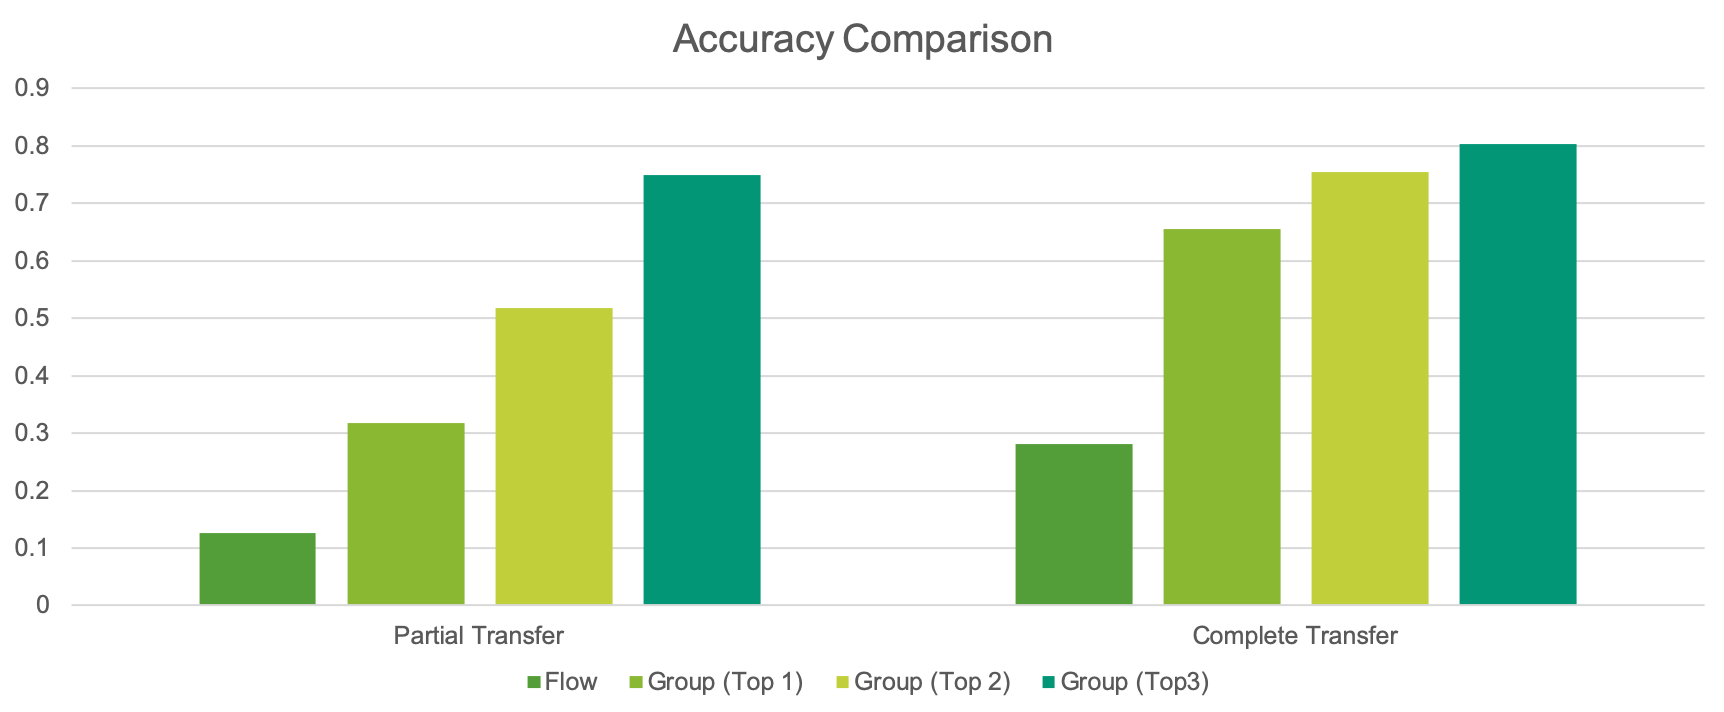
\includegraphics[width=0.45\textwidth]{./figure/dt-result}
\end{center}
\vspace{-0.05in}
\caption{Classification Accuracy with Decision Tree Model}
\vspace{-0.05in}
\label{fig:dt}
\end{figure}

Fig.~\ref{fig:dt} presents the results using the random forest model. The single flow level accuracy is very poor and the accuracy increases dramatically with bigger $k$. It also clearly shows that the model with {\it Complete} data performs much better than the {\it Partial} case. However, the gap becomes small when $k=3$. 

\begin{figure}[!ht]
\begin{center}
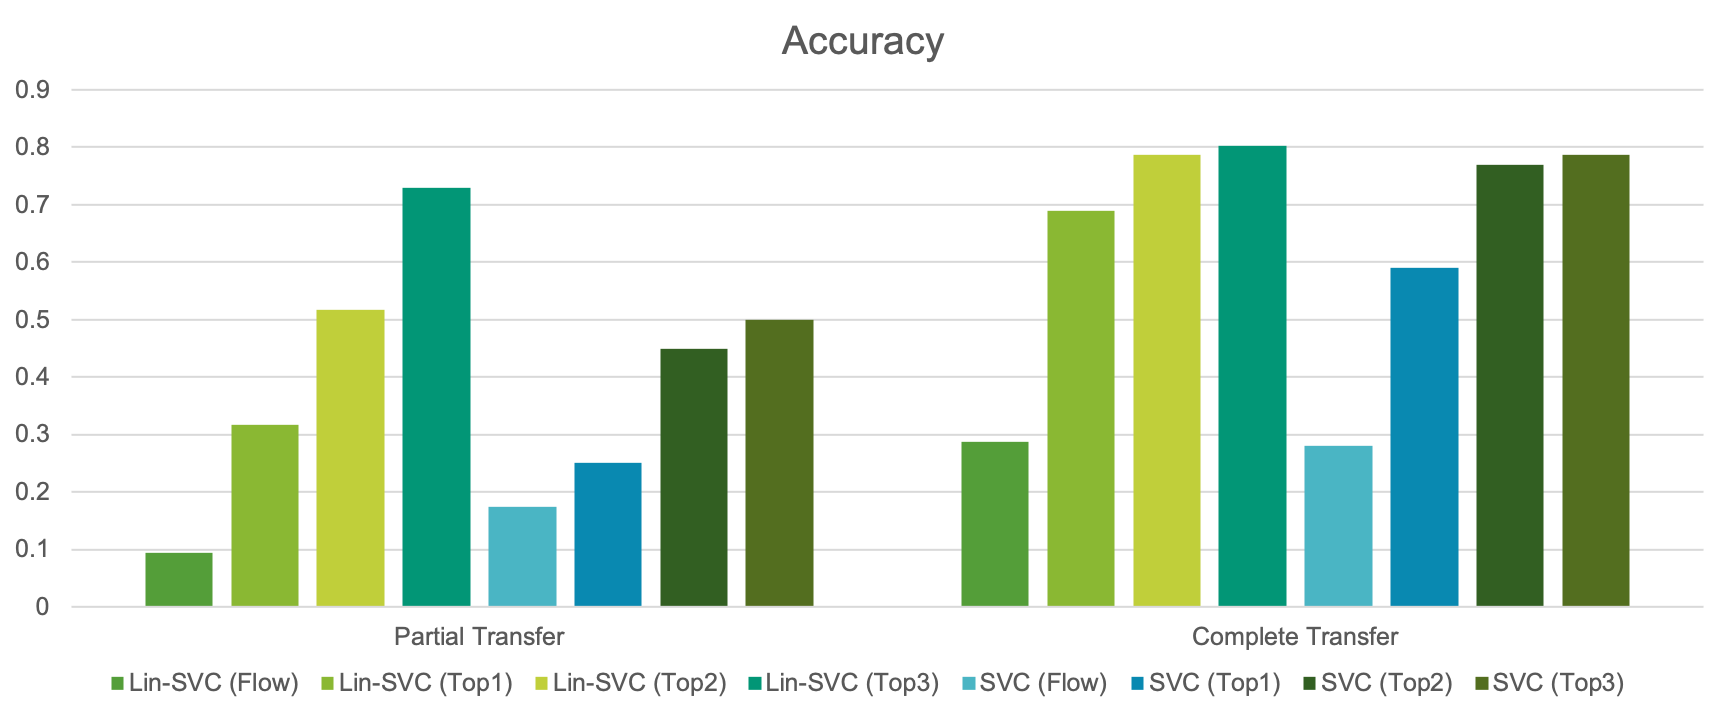
\includegraphics[width=0.45\textwidth]{./figure/svm-result}
\end{center}
\vspace{-0.05in}
\caption{Classification Accuracy with SVM Model}
\vspace{-0.05in}
\label{fig:svm}
\end{figure}

Fig.~\ref{fig:svm} depicts the results using two different models: linear and general SVM with RBF kernel. It shows the same trends with regards to $k$. It also clearly shows that Linear SVM performs better than the general SVM.
\begin{figure}[!ht]
\begin{center}
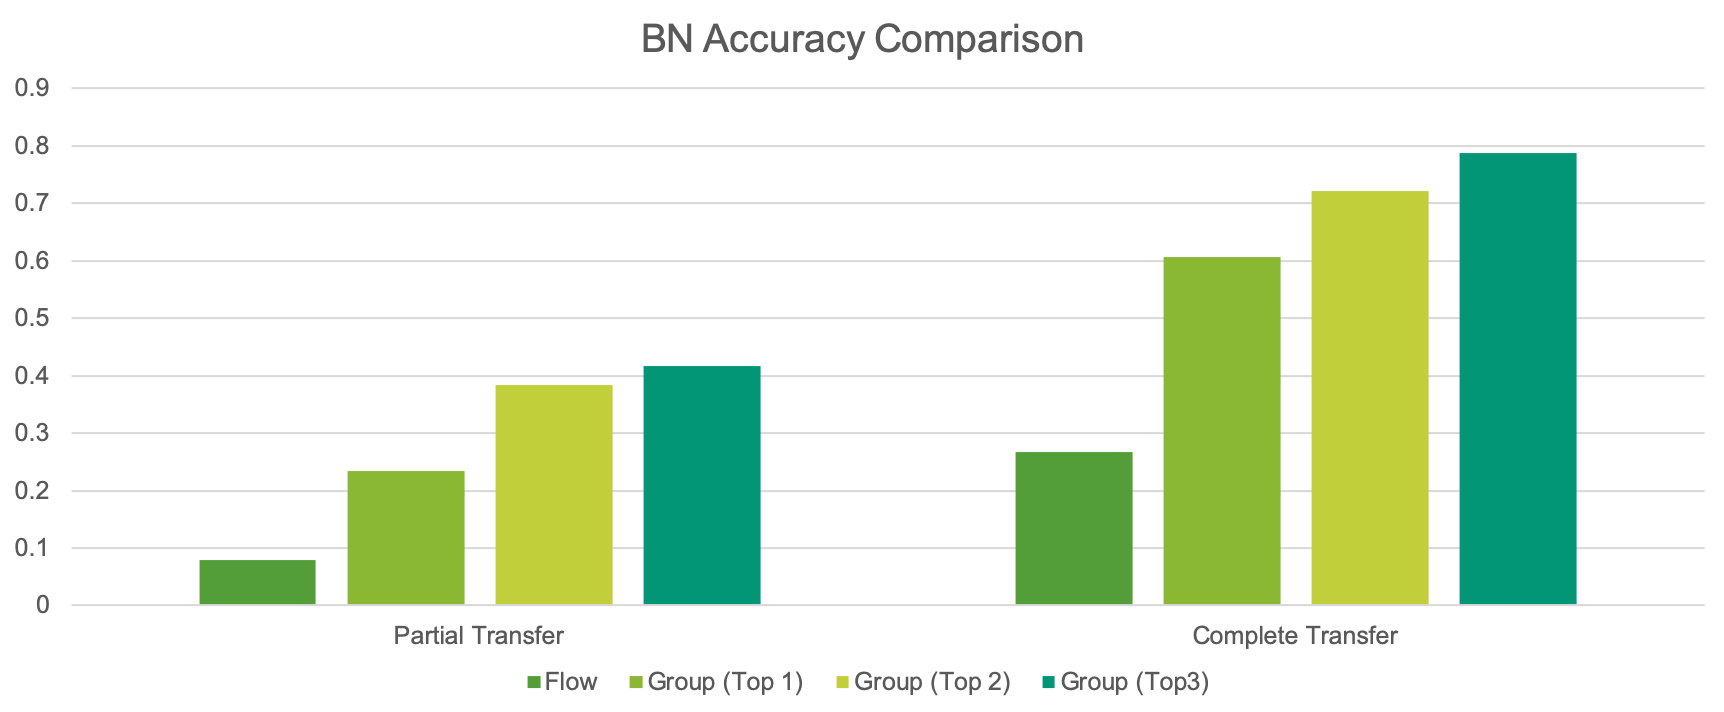
\includegraphics[width=0.45\textwidth]{./figure/bn-result}
\end{center}
\vspace{-0.05in}
\caption{Classification Accuracy with Multinomial Naive Bayes}
\vspace{-0.05in}
\label{fig:bn}
\end{figure}

Fig.~\ref{fig:bn} shows the results using the Multinomial Naive Bayes approach. Again, the accuracy increases with $k$.

When comparing between above three models, the random forest performs the best, linear SVM the next best, and the Bayes model performs the worst. 

When $k=3$, the maximal achieved accuracy is slightly above $80\%$, which is very promising for our specific network RCA problem. We tried larger values of $k$. The accuracy doesn't change much until $k$ reaches 20, when it will jump to above $90\%$. We believe the accuracy stall may be mainly due to the particular topology and more importantly the set of the end hosts for data transfers that do not include all the router nodes, which violates the necessary condition to cover all the possible failure causes in a network~\cite{netbouncer:nsdi18}.  

We next look into the training time of the above three models. From Table.~\ref{tab:time}, it is clear that SVM takes significantly longer time than the other two. Actually the SVC with the default RBF kernel takes much longer time than the linear SVC whose running time is shown in the table. Between the other two, the decision tree model takes the shortest time. Another observation is that the training with the {\it Complete} data set finishes much faster than that with {\it Partial} data set. This makes sense because more complete training data helps the model training converge faster. 

To make the evaluation complete, we also present the F-Score for the single label classification {\it Complete} case in the same table. The SVM model gets the best F-score. As we stated before, we believe the accuracy is the more meaningful metric for the RCA problem, though we will continue to explore better metrics.     
\begin{table}[!ht]
\caption{Training Time and F\-Score
\label{tab:time}}
\vspace{-0.1in}
\begin{center}
\begin{tabular}{ |c|c|c|c| } 
 \hline
  & Partial & Complete & F-Score ($k=1$)\\ 
 \hline\hline
 Decision Tree & 164ms & 95.1ms & 0.3266\\ 
 \hline
 Bayes & 416ms & 174ms & 0.3382 \\
 \hline
 SVM & 26700ms & 10300ms & 0.368 \\ 
 \hline
\end{tabular}
\end{center}
\vspace{-0.1in}
\end{table}
Combining both training accuracy and training time, the random forest model appears to be a clear winner for the studied RCA problem.

\section{Conclusions and Future Work}
\label{sec:future}
We developed a machine learning based network integrity error RCA system that leverages the end-to-end flow monitoring information 
from the application layer, augmented by limited network information. The impacts of different combinations of numerical and categorical data 
features under different realistic network and measurement assumptions on the inference accuracy are quantified via an emulated network created 
in an automated high-fidelity emulation environment we built. The analysis validated that high RCA accuracy to the device level can be achieved with an efficient supervised 
learning model even when only partial network and flow level measurement information are available.

For our future work, we plan to study networks of larger scale with different topology characteristics, more finely tuned ML models, and possible integration with limited network monitoring information. We will further explore the multi-granularity classification framework for large networks. While we focused on single faulty component scenario for integrity errors in this study, we plan to expand to other failure modes and performance degradation RCA systems with multiple concurrent faults. We will also study stochastic approaches that leverage the probability distribution characteristics of the network failures.  


\bibliographystyle{IEEEtran}
\bibliography{iris}

%\newpage
%\begin{appendix} 
%\hfill \break

{\LARGE Demo Description}\\

In order to obtain sufficient amount of training and test data, while guaranteeing experimental repeatability and efficiency, we created a suite of software tools to automate emulation experiments in a Cloud testbed, which can automatically create a large-scale OSPF-enabled virtual network system, initiate data transfers between end hosts, and inject arbitrary integrity errors into the virtual router interfaces and end hosts.  

Our main design objectives is to automate the experiment creation, configuration, and data collection at any given scale. This not only guarantees repeatable experiments at different scales, but also makes data manipulation for ML model training for RCA much more efficient.   

We will demonstrate the three main components of the emulation and RCA analysis system. An emulation experiment in ExoGENI testbed is depicted in Fig.~\ref{fig:chaosjungle}.

\subsection{Network creation and configuration}
An arbitrary topology can be created with nodes in the form of virtual machines (VM) running customized images. We leverage the Postboot scripting capability offered by ExoGENI testbed to automate the network configuration.  

In our experimental topology, we use a set of end hosts to emulate the OSG data sources and sinks, a virtual network consisting of core routers emulating the backbone network service providers (Internet2, ESNet, etc) and access routers emulating the access network service providers (regional research and education networks and campus networks). All nodes are connected with virtual layer-2 links with certain throughput guarantee as the private data plane. An extra management plane interface is also available on every node, which provides remote access from the public Internet. The end hosts run an Ubuntu image with our Chaos Jungle fault injection tools. The routers run an Ubuntu image with the Zebra software router and our Chaos Jungle fault injection tools.

At the virtual node booting time, our customized Postboot scripts automate the following steps: (1) detect all the interfaces and their IP addresses, and all the neighboring nodes and the links; (2) create the configuration files for Zebra and OSPF daemons and start the routing control plane at the router nodes; (3) detect and add the default routes at the end host nodes.    

ExoGENI provides an API to launch any given experimental topology. On a successful execution, our experimental topology will be up and running with routing configured and network reachability established among all end hosts.   

\subsection{Data transfer and fault injection}
For every experiment, we attach a controller node that can reach all the nodes in the topology via the management plane interface. The controller is provided a Postboot script that automatically learns the experimental topology, creates a list of end hosts, routers, and links, and populates the end hosts with a set of files for the data transfer.

A user can log into the controller node, modify the experimental configuration files that define the data origin and sink nodes, the list of nodes to introduce storage integrity error, the list of network link interfaces to be disrupted by the Chaos Jungle tool, and the fault injection probability.

Then the experiment software can be started to inject the fault, transfer the data files from the origins, check the integrity at the sinks, and collect the data. This sequence is repeated for every fault specified in the configuration file.

\begin{figure}[!ht]
\begin{center}
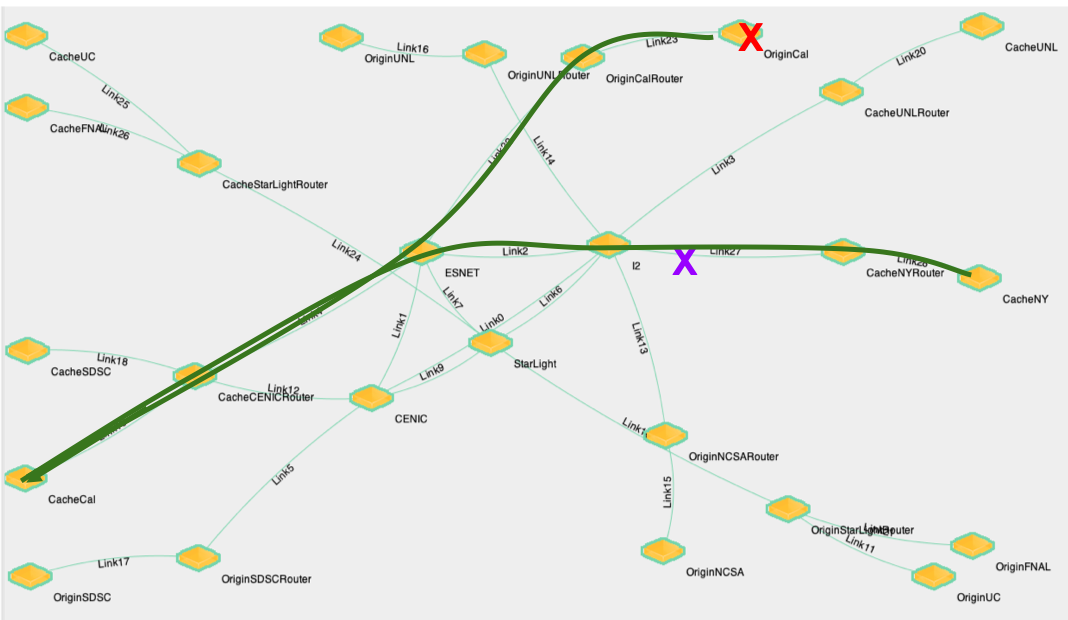
\includegraphics[width=0.48\textwidth]{./figure/ChaosJungle}
\end{center}
\caption{Network Emulation and Integrity Error Injection in ExoGENI}
\label{fig:chaosjungle}
\end{figure}

\subsection{Data collection and analysis}
At the last step, all the raw data will be processed and stored in final result database files with predefined feature columns. Each database entry represents one data transfer with features of file name, file size, origin, sink, access router, integrity error or not, etc. However, the forwarding path is unknown as it is controlled by the routing control plane process. The final result is exported to a Jupyter notebook environment where machine learning based data analysis is performed.

\hfill \break

{\LARGE Demo Set-Up}\\

The default display set-up plus Internet access is sufficient for our demonstration needs as we only run the client at the demo site. The actual experiments will be run in the remote Cloud.


%\end{appendix} 

% That's all folks!
\end{document}
